%=========================================================================
% (c) Michal Bidlo, Bohuslav Křena, 2008

% tikzit regex: (,)?\s*style=\w*(,)?\s*

\listoftodos

\chapter{Introduction}
Nowadays, when malicious code or malware is becoming more and more sophisticated and pressing security risk, it is really needed to control a program behaviour and monitor what the program is doing in a system.
Monitoring program behaviour can be done in many ways and one of the easiest ways is to use Intrusion Detection System (IDS).
IDS is an out-of-the-box solution which can monitor i.e. where program wrote or read something and it is not allowed.
After that, IDS is reporting this violation. %TODO and and

Another way is to monitor and block system calls (syscalls).
Monitoring is performed using tools mentioned in the next chapter.
The actual blocking can be performed with mandatory control access (MAC) (Apparmor, SELinux), sandboxing (seccomp) or others mechanisms.
MAC refers to a type of access control by which the operating system constraints the ability of a subject or initiator to access or generally perform some sort of operation on an object or target.
Seccomp is a Linux kernel module which allows to a process one-way transition to secure a state where the process can only use four syscalls.
When the process tries to call another syscall then one of the four members set is terminated with SIGKILL.
The set of allowed system calls can be extended using seccomp-bpf.
This extension allows filtering system calls using a configurable policy implemented with Berkley Packet Filter (BPF) rules.
This last part is an area on which I would like to focus in my thesis.

I aim to design and develop a tool which helps developers using libseccomp and seccomp-bpf.
I plan to create policies for a specific program in a format readable by libseccomp or seccomp-bpf.

\Cref{chap:syscalls} describes syscalls and how to monitor them.
In the next chapter of the thesis, I will illustrate how security facilities in Linux, such as systrace and seccomp, work.
After the theoretical part, the design and development of a tool will follow.
In conclusion, methodology how this tool was tested is described.

\chapter{System calls and tools monitoring them}
\label{chap:syscalls}
In this chapter, I will describe a term system call and I will make an overview of tools which can monitor the system calls.
We will red focus in detail on a strace tool which will be used as an input to my tool.
The other tools are described briefly not as detailed as strace.

\section{System calls}
System calls or syscalls is a mechanism used by processes to use operating system functions typically in monolithic kernels.
We can find them on every UNIX system.
In computer terminology, the term syscall is the programmatic way in which a computer program requests a service from the kernel of the operating system it is executed on. The system calls are generated using interrupt i.e. on Linux/i86 with interrupt no. \texttt{0x80}. and these syscalls are handled by the kernel in privileged mode.
When a user invokes a system call, execution flow is as follows:
\begin{itemize}
	\item Each call is vectored through a stub in libc. Some system calls are more complex than others because of variable length of arguments. But every syscall has the same entry point and the same exit point. Only overhead in more complex syscalls is processing more parameters on entry.
	\item Each syscall is expanded to assembly routine. This routine also sets up the stack frame and calls \texttt{\_system\_call\(\)} through an interrupt \( \texttt{int \$0x80} \).
	\item There was not executed any code of syscall. Not until int \texttt{\$0x80} is executed, this interrupt does the call transfer to the kernel entry point. The entry point is the same for every system call. Now is saved the state of central process unit (CPU), saved all of the registers, checked if is valid syscall called. Transfering control to a valid syscall is done through the offset in the \texttt{\_sys\_call\_table}.
	\item At the end of the syscall is called \texttt{\_ret\_from\_sys\_call\(\)}. This is done before returning to user space. It checks if the scheduler should be run, and if so, calls it.
	\item Immediately after return from the system call, \texttt{syscallX()} macro checks for a negative return value from the syscall, if so it puts a positive copy to a global variable \texttt{\_errno}, for accessing from code like \texttt{perror()}.

	\todo{Decide which one}

	\item Each syscall is vectored through a stub in libc. Some syscalls are more complex than others because of variable length of arguments, but the entry point and end point of syscall is still the same. Only overhead is processing more arguments.
	\item In libc is then set the number of the syscall to \texttt{eax} register and the stack frame is also set up.
	\item Interrupt number \texttt{0x80} is called and transfered to kernel entry point. The entry point is the same for every system call.
	\item In table of interrupts is found a pointer to interrupt handler. After that follows the execution of the interrupt handler. Now in the handler is stored the content of the CPU registers, checked if is valid syscall called.
	\item The handler finds the corresponding offset in table of interrupts \texttt{\_sys\_call\_table}, where is stored pointer to syscall service.
	\item Control is transfered to the syscall service.
	\item Syscall returned return value to register \texttt{EAX} on 32-bit architecture or \texttt{RAX} on 64-bit architecture.
	\item At the end of the syscall is called \texttt{\_ret\_from\_sys\_call\(\)}. This is done before returning to user space. It checks if the scheduler should be run, and if so, calls it.
	\item Immediately after return from the system call to interrupt handler, \texttt{syscallX()} macro checks for a negative return value from the syscall, if so it puts a positive copy to a global variable \texttt{\_errno}, for accessing from code like \texttt{perror()}.
\end{itemize}

\missingfigure{Make a sketch of the calling a syscall}

\begin{figure}
  \center
  % \includestandalone[width=\textwidth]{obrazky-figures/mytikz}%     without .tex extension
  \begin{tikzpicture}[align=left, thick]
	\begin{pgfonlayer}{nodelayer}
		\node [] (0) at (-5, 5) {};
		\node [] (1) at (-4, 5) {};
		\node [] (2) at (-5, 3.75) {};
		\node [] (3) at (-4, 3.75) {};
		\node [] (4) at (-2, 6) {};
		\node [] (5) at (-2, 3.25) {};
		\node [] (6) at (1, 3.25) {};
		\node [] (7) at (1, 6) {};
		\node [] (8) at (-4, 4.5) {};
		\node [] (9) at (-4, 4.25) {};
		\node [] (10) at (-2, 4.5) {};
		\node [] (11) at (-2, 4.25) {};
		\node [] (12) at (-5, 4.5) {};
		\node [] (13) at (-6, 4.5) {};
		\node [] (14) at (-6, 2) {};
		\node [] (15) at (-8, 2) {};
		\node [] (16) at (2.25, 2) {};
		\node [] (17) at (-6, 1) {};
		\node [] (18) at (-8, 1) {};
		\node [] (19) at (-6.25, 1) {};
		\node [] (20) at (-5.75, 1) {};
		\node [] (21) at (-4.25, 1) {};
		\node [] (22) at (-4.25, -0) {};
		\node [] (23) at (-5.75, -0) {};
		\node [] (24) at (-6, -0) {};
		\node [] (25) at (-6.25, -0) {};
		\node [] (26) at (-8, -0) {};
		\node [] (27) at (-6, 0.5) {};
		\node [] (28) at (-4.5, -0.75) {};
		\node [] (29) at (-4.5, -1.75) {};
		\node [] (30) at (-3.5, -1.75) {};
		\node [] (31) at (-3.5, -0.75) {};
		\node [] (32) at (-4, -1.25) {};
		\node [] (33) at (-4.5, -1.25) {};
		\node [] (34) at (-2, -0) {};
		\node [] (35) at (-2, -2.5) {};
		\node [] (36) at (-1, -2.5) {};
		\node [] (37) at (-1, -0) {};
		\node [] (38) at (-2, -0.75) {};
		\node [] (39) at (-1, -0.75) {};
		\node [] (40) at (-1, -1.25) {};
		\node [] (41) at (-2, -1.25) {};
		\node [] (42) at (0, -0) {};
		\node [] (43) at (1, -0) {};
		\node [] (44) at (1, -1) {};
		\node [] (45) at (0, -1) {};
		\node [] (46) at (0, -1.75) {};
		\node [] (47) at (1, -1.75) {};
		\node [] (48) at (1, -2.75) {};
		\node [] (49) at (0, -2.75) {};
		\node [] (50) at (-1.5, -1) {};
		\node [] (51) at (0, -0.5) {};
		\node [] (52) at (-2, -1) {};
		\node [] (53) at (-3.75, -0.5) {};
		\node [] (54) at (0.5, -0) {};
		\node [] (55) at (-4, -0.5) {};
		\node [] (56) at (-4.25, 3.5) {};
		\node [font={\tiny}, right, align=left,] (57) at (-7.75, 2.25) {User space};
		\node [font={\tiny}, right, align=left,] (58) at (-7.75, 1.75) {Kernel space};
		\node [align=left, rotate=270, font=\small] (59) at (-5.75, 3) {\texttt{int \$0x80}};
		\node [] (60) at (-4.5, 5.25) {libc};
		\node [] (61) at (-0.5, 6.25) {source.c};
		\node [font={\small}, align=left,] (62) at (-0.75, 5.5) {int main()\{};
		\node [font={\small}, align=left,] (63) at (-0.25, 5) {printf("42")\;};
		\node [font={\small}, align=left,] (64) at (-0.5, 4.5) {return 0;};
		\node [font={\small}, align=left,] (65) at (-1.5, 4) {\}};
		\node [] (66) at (-4, -2.25) {};
	\end{pgfonlayer}
	\begin{pgfonlayer}{edgelayer}
		\draw [] (0.center) to (1.center);
		\draw [] (0.center) to (2.center);
		\draw [] (2.center) to (3.center);
		\draw [] (3.center) to (9.center);
		\draw [] (9.center) to (8.center);
		\draw [] (8.center) to (1.center);
		\draw [->, thick] (8.center) to (10.center);
		\draw [<-, loosely dashed, thick, in=180, out=0, looseness=1.00] (9.center) to (11.center);
		\draw [] (11.center) to (10.center);
		\draw [] (4.center) to (10.center);
		\draw [] (5.center) to (11.center);
		\draw [] (5.center) to (6.center);
		\draw [] (6.center) to (7.center);
		\draw [] (7.center) to (4.center);
		\draw [thick,] (12.center) to (13.center);
		\draw [thick,] (13.center) to (14.center);
		\draw [ultra thick,] (14.center) to (15.center);
		\draw [, ultra thick] (14.center) to (16.center);
		\draw [thick, ->] (14.center) to (17.center);
		\draw [] (17.center) to (20.center);
		\draw [] (20.center) to (21.center);
		\draw [] (22.center) to (23.center);
		\draw [] (20.center) to (23.center);
		\draw [] (23.center) to (24.center);
		\draw [] (24.center) to (25.center);
		\draw [] (25.center) to (19.center);
		\draw [] (19.center) to (17.center);
		\draw [] (19.center) to (18.center);
		\draw [] (18.center) to (26.center);
		\draw [] (26.center) to (25.center);
		\draw [] (28.center) to (33.center);
		\draw [] (33.center) to (29.center);
		\draw [] (29.center) to (30.center);
		\draw [] (31.center) to (28.center);
		\draw [thick, ->, in=180, out=-90, looseness=1.25] (27.center) to (33.center);
		\draw [] (38.center) to (41.center);
		\draw [] (41.center) to (40.center);
		\draw [] (40.center) to (39.center);
		\draw [] (39.center) to (38.center);
		\draw [] (38.center) to (34.center);
		\draw [] (34.center) to (37.center);
		\draw [] (37.center) to (39.center);
		\draw [] (40.center) to (36.center);
		\draw [] (41.center) to (35.center);
		\draw [] (49.center) to (48.center);
		\draw [] (48.center) to (47.center);
		\draw [] (47.center) to (46.center);
		\draw [] (46.center) to (49.center);
		\draw [] (45.center) to (44.center);
		\draw [] (44.center) to (43.center);
		\draw [] (43.center) to (42.center);
		\draw [] (42.center) to (45.center);
		\draw [thick, ->, loosely dashed, in=-60, out=75, looseness=1.00] (55.center) to (56.center);
		\draw [thick, ->, in=180, out=0, looseness=1.00] (32.center) to node[font={\small}, align=center, above=2pt]{\texttt{eax}} (52.center);
		\draw [thick, loosely dashed, ->, in=75, out=120, looseness=1.00] (54.center) to (53.center);
		\draw [] (31.center) to (30.center);
		\draw [->, thick, in=180, out=0, looseness=1.00] (50.center) to (51.center);
	\end{pgfonlayer}
\end{tikzpicture}
  \caption{Interrupt handling}
  \label{fig:tikz:int_handling}
\end{figure}

\todo[color=green, inline]{Make description to the above figure \ldots}

% % Graphic for TeX using PGF
% Title: /home/mtamasko/School/IBP/obrazky-figures/Diagram1.dia
% Creator: Dia v0.97.3
% CreationDate: Mon Oct 23 15:11:28 2017
% For: mtamasko
% \usepackage{tikz}
% The following commands are not supported in PSTricks at present
% We define them conditionally, so when they are implemented,
% this pgf file will use them.
\ifx\du\undefined
  \newlength{\du}
\fi
\setlength{\du}{15\unitlength}
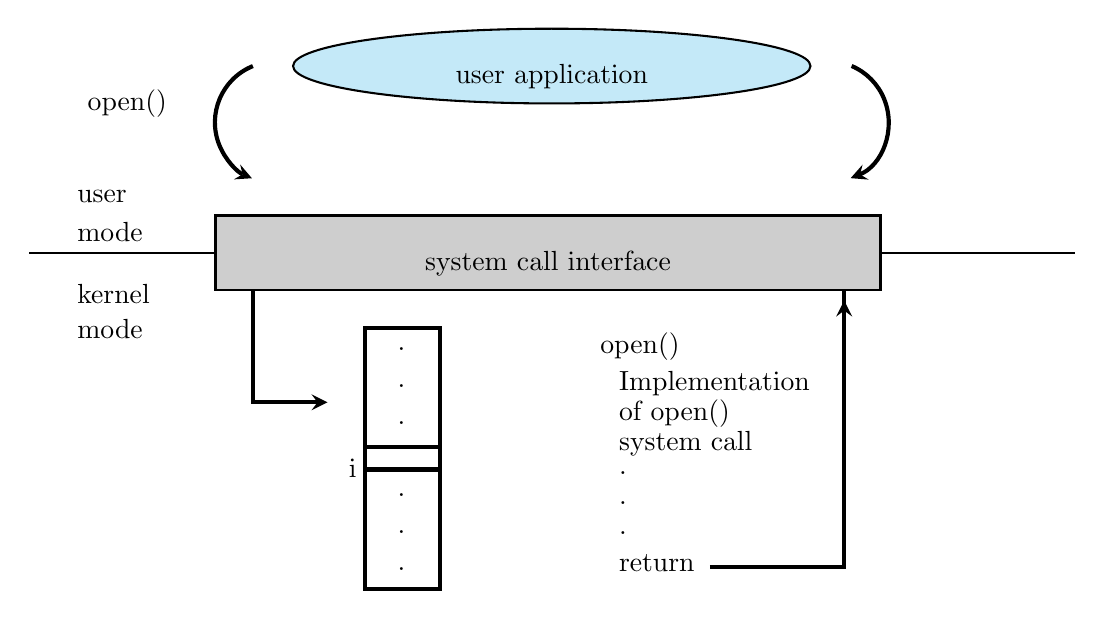
\begin{tikzpicture}
\pgftransformxscale{0.900000}
\pgftransformyscale{-0.900000}
\definecolor{dialinecolor}{rgb}{0.000000, 0.000000, 0.000000}
\pgfsetstrokecolor{dialinecolor}
\definecolor{dialinecolor}{rgb}{1.000000, 1.000000, 1.000000}
\pgfsetfillcolor{dialinecolor}
\pgfsetlinewidth{0.050000\du}
\pgfsetdash{}{0pt}
\pgfsetdash{}{0pt}
\pgfsetmiterjoin
\definecolor{dialinecolor}{rgb}{0.807843, 0.807843, 0.807843}
\pgfsetfillcolor{dialinecolor}
\fill (35.500000\du,7.000000\du)--(35.500000\du,9.000000\du)--(53.300000\du,9.000000\du)--(53.300000\du,7.000000\du)--cycle;
\definecolor{dialinecolor}{rgb}{0.000000, 0.000000, 0.000000}
\pgfsetstrokecolor{dialinecolor}
\draw (35.500000\du,7.000000\du)--(35.500000\du,9.000000\du)--(53.300000\du,9.000000\du)--(53.300000\du,7.000000\du)--cycle;
\pgfsetlinewidth{0.050000\du}
\pgfsetdash{}{0pt}
\pgfsetdash{}{0pt}
\pgfsetbuttcap
{
\definecolor{dialinecolor}{rgb}{0.000000, 0.000000, 0.000000}
\pgfsetfillcolor{dialinecolor}
% was here!!!
\definecolor{dialinecolor}{rgb}{0.000000, 0.000000, 0.000000}
\pgfsetstrokecolor{dialinecolor}
\draw (35.500000\du,8.000000\du)--(30.500000\du,8.000000\du);
}
\pgfsetlinewidth{0.050000\du}
\pgfsetdash{}{0pt}
\pgfsetdash{}{0pt}
\pgfsetbuttcap
{
\definecolor{dialinecolor}{rgb}{0.000000, 0.000000, 0.000000}
\pgfsetfillcolor{dialinecolor}
% was here!!!
\definecolor{dialinecolor}{rgb}{0.000000, 0.000000, 0.000000}
\pgfsetstrokecolor{dialinecolor}
\draw (58.500000\du,8.000000\du)--(53.300000\du,8.000000\du);
}
\definecolor{dialinecolor}{rgb}{0.768627, 0.913725, 0.972549}
\pgfsetfillcolor{dialinecolor}
\pgfpathellipse{\pgfpoint{44.500000\du}{3.000000\du}}{\pgfpoint{6.925000\du}{0\du}}{\pgfpoint{0\du}{1.000000\du}}
\pgfusepath{fill}
\pgfsetlinewidth{0.050000\du}
\pgfsetdash{}{0pt}
\pgfsetdash{}{0pt}
\definecolor{dialinecolor}{rgb}{0.000000, 0.000000, 0.000000}
\pgfsetstrokecolor{dialinecolor}
\pgfpathellipse{\pgfpoint{44.500000\du}{3.000000\du}}{\pgfpoint{6.925000\du}{0\du}}{\pgfpoint{0\du}{1.000000\du}}
\pgfusepath{stroke}
\pgfsetlinewidth{0.100000\du}
\pgfsetdash{}{0pt}
\pgfsetdash{}{0pt}
\pgfsetbuttcap
{
\definecolor{dialinecolor}{rgb}{0.000000, 0.000000, 0.000000}
\pgfsetfillcolor{dialinecolor}
% was here!!!
\pgfsetarrowsend{stealth}
\definecolor{dialinecolor}{rgb}{0.000000, 0.000000, 0.000000}
\pgfsetstrokecolor{dialinecolor}
\pgfpathmoveto{\pgfpoint{36.500049\du}{2.999979\du}}
\pgfpatharc{248}{113}{1.625000\du and 1.625000\du}
\pgfusepath{stroke}
}
\pgfsetlinewidth{0.100000\du}
\pgfsetdash{}{0pt}
\pgfsetdash{}{0pt}
\pgfsetbuttcap
{
\definecolor{dialinecolor}{rgb}{0.000000, 0.000000, 0.000000}
\pgfsetfillcolor{dialinecolor}
% was here!!!
\pgfsetarrowsstart{stealth}
\definecolor{dialinecolor}{rgb}{0.000000, 0.000000, 0.000000}
\pgfsetstrokecolor{dialinecolor}
\pgfpathmoveto{\pgfpoint{52.499872\du}{6.000053\du}}
\pgfpatharc{68}{-67}{1.625000\du and 1.625000\du}
\pgfusepath{stroke}
}
% setfont left to latex
\definecolor{dialinecolor}{rgb}{0.000000, 0.000000, 0.000000}
\pgfsetstrokecolor{dialinecolor}
\node at (44.500000\du,3.275000\du){user application};
% setfont left to latex
\definecolor{dialinecolor}{rgb}{0.000000, 0.000000, 0.000000}
\pgfsetstrokecolor{dialinecolor}
\node at (44.400000\du,8.283750\du){system call interface};
% setfont left to latex
\definecolor{dialinecolor}{rgb}{0.000000, 0.000000, 0.000000}
\pgfsetstrokecolor{dialinecolor}
\node[anchor=east] at (34.500000\du,4.000000\du){open()};
% setfont left to latex
\definecolor{dialinecolor}{rgb}{0.000000, 0.000000, 0.000000}
\pgfsetstrokecolor{dialinecolor}
\node[anchor=west] at (31.500000\du,6.486825\du){user};
% setfont left to latex
\definecolor{dialinecolor}{rgb}{0.000000, 0.000000, 0.000000}
\pgfsetstrokecolor{dialinecolor}
\node[anchor=west] at (31.500000\du,7.445675\du){mode};
% setfont left to latex
\definecolor{dialinecolor}{rgb}{0.000000, 0.000000, 0.000000}
\pgfsetstrokecolor{dialinecolor}
\node[anchor=west] at (31.500000\du,9.086825\du){kernel};
% setfont left to latex
\definecolor{dialinecolor}{rgb}{0.000000, 0.000000, 0.000000}
\pgfsetstrokecolor{dialinecolor}
\node[anchor=west] at (31.500000\du,10.045675\du){mode};
\pgfsetlinewidth{0.100000\du}
\pgfsetdash{}{0pt}
\pgfsetdash{}{0pt}
\pgfsetmiterjoin
\pgfsetbuttcap
{
\definecolor{dialinecolor}{rgb}{0.000000, 0.000000, 0.000000}
\pgfsetfillcolor{dialinecolor}
% was here!!!
\pgfsetarrowsend{stealth}
{\pgfsetcornersarced{\pgfpoint{0.000000\du}{0.000000\du}}\definecolor{dialinecolor}{rgb}{0.000000, 0.000000, 0.000000}
\pgfsetstrokecolor{dialinecolor}
\draw (36.500000\du,9.000000\du)--(36.500000\du,9.000000\du)--(36.500000\du,12.000000\du)--(38.500000\du,12.000000\du);
}}
\pgfsetlinewidth{0.100000\du}
\pgfsetdash{}{0pt}
\pgfsetdash{}{0pt}
\pgfsetmiterjoin
\definecolor{dialinecolor}{rgb}{1.000000, 1.000000, 1.000000}
\pgfsetfillcolor{dialinecolor}
\fill (39.500000\du,10.000000\du)--(39.500000\du,17.000000\du)--(41.500000\du,17.000000\du)--(41.500000\du,10.000000\du)--cycle;
\definecolor{dialinecolor}{rgb}{0.000000, 0.000000, 0.000000}
\pgfsetstrokecolor{dialinecolor}
\draw (39.500000\du,10.000000\du)--(39.500000\du,17.000000\du)--(41.500000\du,17.000000\du)--(41.500000\du,10.000000\du)--cycle;
% setfont left to latex
\definecolor{dialinecolor}{rgb}{0.000000, 0.000000, 0.000000}
\pgfsetstrokecolor{dialinecolor}
\node[anchor=west] at (40.070054\du,10.577100\du){.};
% setfont left to latex
\definecolor{dialinecolor}{rgb}{0.000000, 0.000000, 0.000000}
\pgfsetstrokecolor{dialinecolor}
\node[anchor=west] at (40.070054\du,11.564878\du){.};
% setfont left to latex
\definecolor{dialinecolor}{rgb}{0.000000, 0.000000, 0.000000}
\pgfsetstrokecolor{dialinecolor}
\node[anchor=west] at (40.070054\du,12.552655\du){.};
% setfont left to latex
\definecolor{dialinecolor}{rgb}{0.000000, 0.000000, 0.000000}
\pgfsetstrokecolor{dialinecolor}
\node[anchor=west] at (40.070054\du,14.484400\du){.};
% setfont left to latex
\definecolor{dialinecolor}{rgb}{0.000000, 0.000000, 0.000000}
\pgfsetstrokecolor{dialinecolor}
\node[anchor=west] at (40.070054\du,15.472178\du){.};
% setfont left to latex
\definecolor{dialinecolor}{rgb}{0.000000, 0.000000, 0.000000}
\pgfsetstrokecolor{dialinecolor}
\node[anchor=west] at (40.070054\du,16.459955\du){.};
\pgfsetlinewidth{0.100000\du}
\pgfsetdash{}{0pt}
\pgfsetdash{}{0pt}
\pgfsetbuttcap
{
\definecolor{dialinecolor}{rgb}{0.000000, 0.000000, 0.000000}
\pgfsetfillcolor{dialinecolor}
% was here!!!
\definecolor{dialinecolor}{rgb}{0.000000, 0.000000, 0.000000}
\pgfsetstrokecolor{dialinecolor}
\draw (39.500000\du,13.200000\du)--(41.500000\du,13.200000\du);
}
\pgfsetlinewidth{0.100000\du}
\pgfsetdash{}{0pt}
\pgfsetdash{}{0pt}
\pgfsetbuttcap
{
\definecolor{dialinecolor}{rgb}{0.000000, 0.000000, 0.000000}
\pgfsetfillcolor{dialinecolor}
% was here!!!
\definecolor{dialinecolor}{rgb}{0.000000, 0.000000, 0.000000}
\pgfsetstrokecolor{dialinecolor}
\draw (39.500000\du,13.800000\du)--(41.500000\du,13.800000\du);
}
% setfont left to latex
\definecolor{dialinecolor}{rgb}{0.000000, 0.000000, 0.000000}
\pgfsetstrokecolor{dialinecolor}
\node[anchor=west] at (38.770000\du,13.765600\du){i};
% setfont left to latex
\definecolor{dialinecolor}{rgb}{0.000000, 0.000000, 0.000000}
\pgfsetstrokecolor{dialinecolor}
\node[anchor=west] at (45.500000\du,10.500000\du){open()};
% setfont left to latex
\definecolor{dialinecolor}{rgb}{0.000000, 0.000000, 0.000000}
\pgfsetstrokecolor{dialinecolor}
\node[anchor=west] at (46.000000\du,11.500000\du){Implementation};
% setfont left to latex
\definecolor{dialinecolor}{rgb}{0.000000, 0.000000, 0.000000}
\pgfsetstrokecolor{dialinecolor}
\node[anchor=west] at (46.000000\du,12.300000\du){of open()};
% setfont left to latex
\definecolor{dialinecolor}{rgb}{0.000000, 0.000000, 0.000000}
\pgfsetstrokecolor{dialinecolor}
\node[anchor=west] at (46.000000\du,13.100000\du){system call};
% setfont left to latex
\definecolor{dialinecolor}{rgb}{0.000000, 0.000000, 0.000000}
\pgfsetstrokecolor{dialinecolor}
\node[anchor=west] at (46.000000\du,13.900000\du){  .};
% setfont left to latex
\definecolor{dialinecolor}{rgb}{0.000000, 0.000000, 0.000000}
\pgfsetstrokecolor{dialinecolor}
\node[anchor=west] at (46.000000\du,14.700000\du){  .};
% setfont left to latex
\definecolor{dialinecolor}{rgb}{0.000000, 0.000000, 0.000000}
\pgfsetstrokecolor{dialinecolor}
\node[anchor=west] at (46.000000\du,15.500000\du){  .};
% setfont left to latex
\definecolor{dialinecolor}{rgb}{0.000000, 0.000000, 0.000000}
\pgfsetstrokecolor{dialinecolor}
\node[anchor=west] at (46.000000\du,16.300000\du){return};
\pgfsetlinewidth{0.100000\du}
\pgfsetdash{}{0pt}
\pgfsetdash{}{0pt}
\pgfsetmiterjoin
\pgfsetbuttcap
{
\definecolor{dialinecolor}{rgb}{0.000000, 0.000000, 0.000000}
\pgfsetfillcolor{dialinecolor}
% was here!!!
\pgfsetarrowsend{stealth}
{\pgfsetcornersarced{\pgfpoint{0.000000\du}{0.000000\du}}\definecolor{dialinecolor}{rgb}{0.000000, 0.000000, 0.000000}
\pgfsetstrokecolor{dialinecolor}
\draw (48.733774\du,16.409121\du)--(52.327092\du,16.409121\du)--(52.327092\du,9.273381\du)--(52.327092\du,9.273381\du);
}}
\end{tikzpicture}


\section{Monitoring}
The most used method for monitoring is tracing, in other words watching what a program is doing. Tracing involves a specialized logging to record information, useful for debugging, about a program's execution. This can be done in multiple layers, from tracing which lines in the program was executed to individual instructions executed on CPU. Collecting of this information can be done with multiple tools i.e strace, ftrace and a lot more.

\subsection{Strace -- trace system calls and signals}
\subsection{Ftrace -- trace system calls, function calls and signals}
\subsection{Ltrace}
\subsection{Dtrace}
\subsection{Autrace -- linux audit}

\chapter{Security facility in Linux}
Systrace and seccomp\cite{Pravidla}
\section{Systrace}
123

\section{Seccomp}
321
\subsection{Seccomp-bpf}

\subsection{Berkeley packet filter}
\subsubsection{Classic BPF}
\subsubsection{Extended BPF}

\subsection{libseccomp}


\chapter{Development of TODO: tool-name}
\section{Input}
\section{Intermediate representation}
\section{Output}
\section{Heuristics and optimizations}
\subsection{Minimax}
\subsection{Strict}
\subsection{Smart}


\chapter{Testing methods}


%=========================================================================
